\documentclass[12pt]{article}
	
\usepackage[margin=1in]{geometry}		% For setting margins
\usepackage{amsmath}				% For Math
\usepackage{fancyhdr}				% For fancy header/footer
\usepackage{graphicx}				% For including figure/image
\usepackage{cancel}					% To use the slash to cancel out stuff in work

%%%%%%%%%%%%%%%%%%%%%%
% Set up fancy header/footer
\pagestyle{fancy}
\fancyhead[LO,L]{Kate O'Neill - 213 657 68}
\fancyhead[CO,C]{CSU11031 Assignment IV}
\fancyhead[RO,R]{\today}
\fancyfoot[LO,L]{}
\fancyfoot[CO,C]{\thepage}
\fancyfoot[RO,R]{}
\renewcommand{\headrulewidth}{0.4pt}
\renewcommand{\footrulewidth}{0.4pt}
%%%%%%%%%%%%%%%%%%%%%%

\usepackage{listings}
\usepackage{xcolor}

\definecolor{codegreen}{rgb}{0,0.6,0}
\definecolor{codegray}{rgb}{0.5,0.5,0.5}
\definecolor{codepurple}{rgb}{0.58,0,0.82}
\definecolor{backcolour}{rgb}{0.95,0.95,0.92}

\lstdefinestyle{mystyle}{
    backgroundcolor=\color{backcolour},   
    commentstyle=\color{codegreen},
    keywordstyle=\color{magenta},
    numberstyle=\tiny\color{codegray},
    stringstyle=\color{codepurple},
    basicstyle=\ttfamily\footnotesize,
    breakatwhitespace=false,         
    breaklines=true,                 
    captionpos=b,                    
    keepspaces=true,                 
    numbers=left,                    
    numbersep=5pt,                  
    showspaces=false,                
    showstringspaces=false,
    showtabs=false,                  
    tabsize=2
}

\lstset{style=mystyle}

\begin{document}
\noindent 1.) The square wave: build a 6 subplot figure to show the time domain, and use respectively 1, 3, 5, 10, 50, 500 frequencies.\\
\begin{figure}[!h] 
	\begin{centering}
		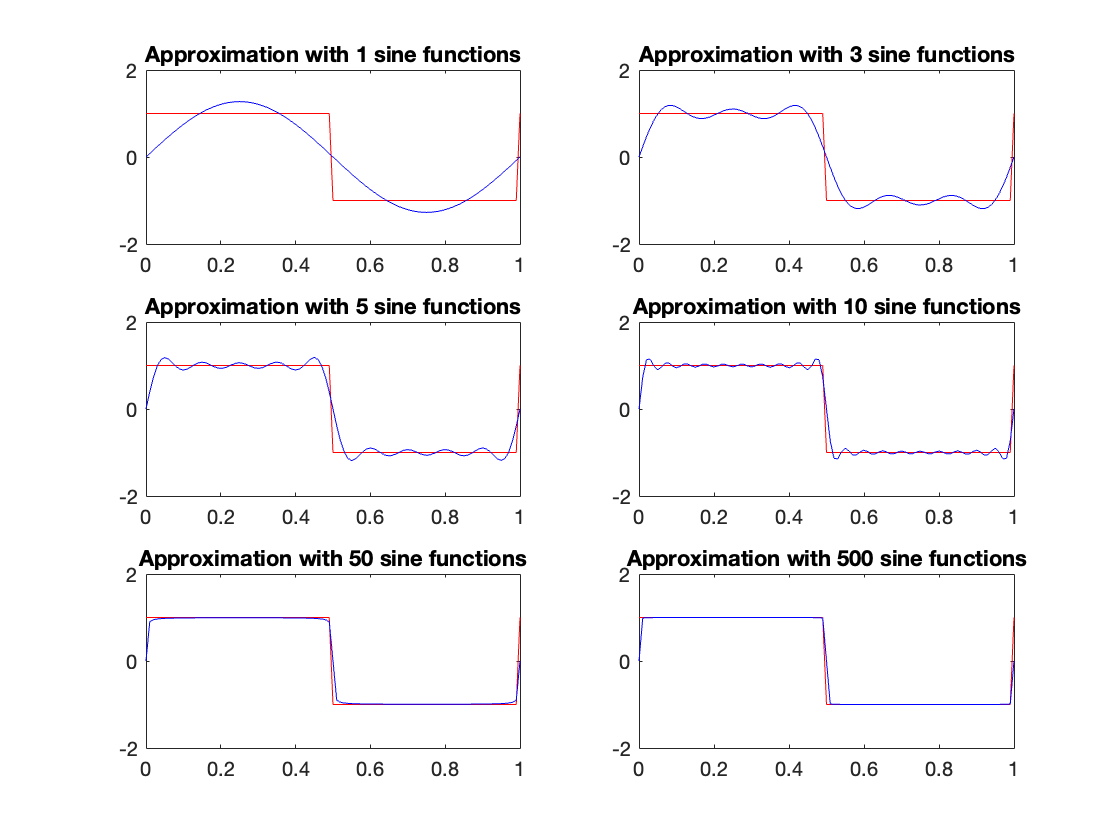
\includegraphics[keepaspectratio = true, width = 7in]{part1.png}
		\caption{Square wave approximation in time}
	\end{centering}
\end{figure}\\
\lstinputlisting[language=Octave]{one.m}\\
\noindent 2.) You should then draw the plot showing all sine components up to 10 sine functions overlapping in a single plot.\\
\begin{figure}[!h] 
	\begin{centering}
		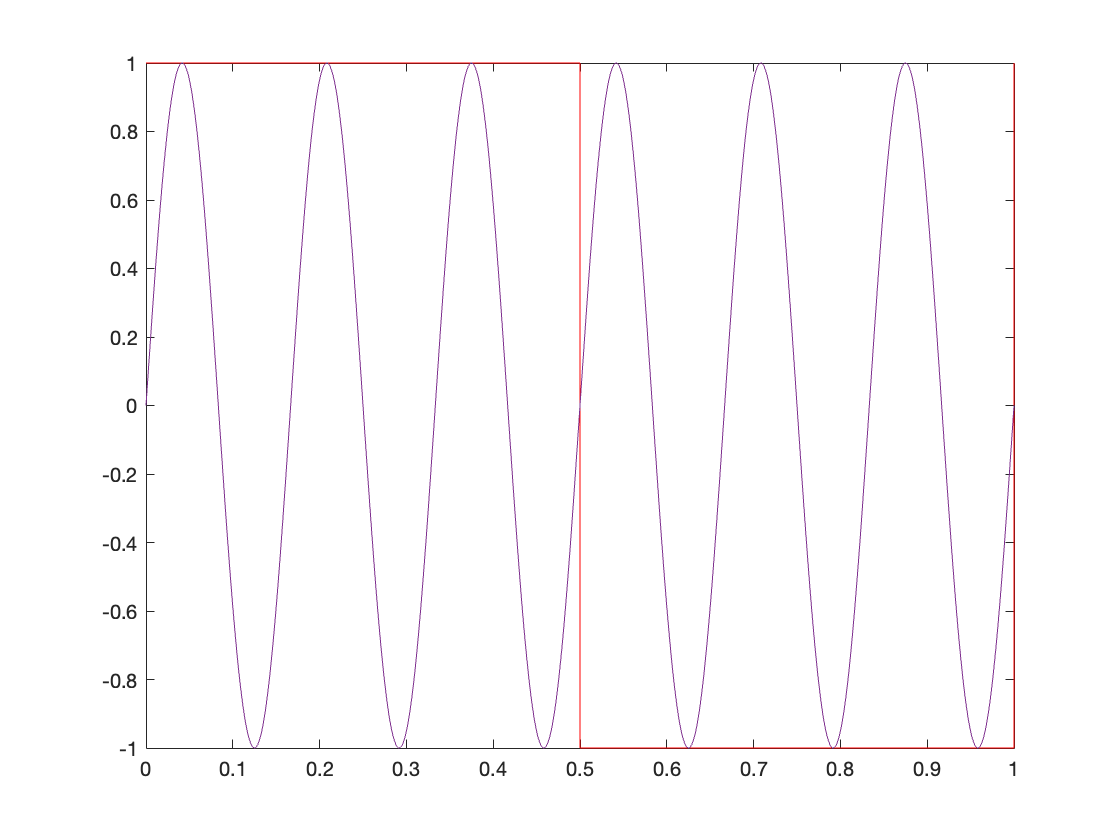
\includegraphics[keepaspectratio = true, width = 7in]{two.png}
		\caption{Sine function overlapping in time}
	\end{centering}
	\lstinputlisting[language=Octave]{two.m}\\
\end{figure}\\
\noindent 3.) Draw the representation in the frequency domain of the square wave approximation in exercise 1). \\
\begin{figure}[!h] 
	\begin{centering}
		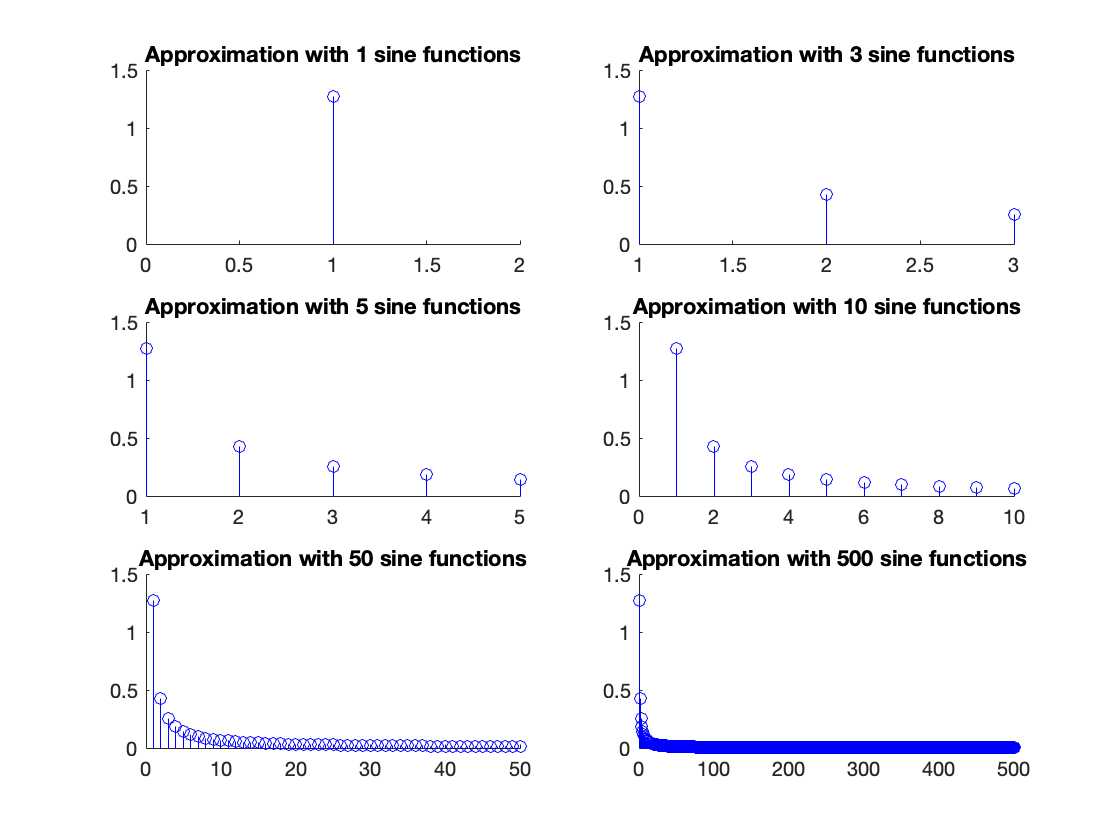
\includegraphics[keepaspectratio = true, width = 7in]{three.png}
		\caption{Square wave approximation in frequency}
	\end{centering}
\end{figure}\\
\lstinputlisting[language=Octave]{three.m}
\end{document}